\scanpage{57}
$F_{\unsure{o|0}}$ le Module qu'il induit sur $X_o$. On suppose \quad a) Pour tout $s\quad S$, la section $t_s$ induite par $t$ sur la fibre $X_s$ est $\underline{O}_{X_s}$-régulière et $\underline{F}_s$-régulière \quad b) $\underline{F}$ et $\underline{O}_X$ sont plats par rapport à $S$ \quad c) Pour tout $s\quad S$, $F_{o\ s}$, \deleted{et} $\underline{O}_{X_{o\ s}}$ \inserted{et $\underline{O}_{X_s}$} sont de profondeur $\quad 2$ en les points fermés de $X_{\deleted{\unsure{o|0}}s\ \deleted{s}}$. Sous ces conditions, il existe un Module cohérent $F$ sur $X$, et un isomorphisme de son complété formel $\widehat{F}$ le long de $X_o$ avec $\underline F$.

Cet énoncé va résulter du suivant:

\uline{Corollaire} 3.2. \quad Sous les conditions de 3\unsure{;|.}1. \quad (

\[
\handwritten{\coprod_{\substack{p\geq\unsure{p|0|p_0}\\ q\geq0}}F_0(q-p)}
\]
\[
\handwritten{M+M(1)+\text{- -}+M(-p)}
\qquad
\handwritten{\coprod_{0,q}S_q}
\]
\figure{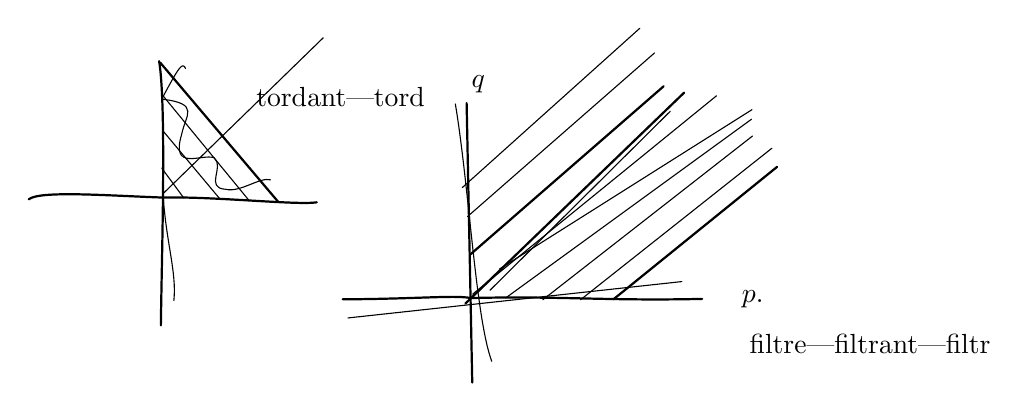
\begin{tikzpicture}[x=.55cm,y=.55cm,line cap=round,line join=round]
\draw[thick] (-3.1,-.04) .. controls (-2.85,.17) and (-1.2,.04) .. (0,0) .. controls (1.15,.03) and (3.1,-.18) .. (3.55,-.11);
\draw[thick] (-.09,3.15) .. controls (.08,2.1) and (-.03,-1.3) .. (-.05,-2.95);
\draw (0,.1) .. controls (.06,-1) and (.32,-1.72) .. (.25,-2.38);
\draw (-.03,.68)--(.48,-.01);
\draw (-.01,1.55)--(1.32,-.04);
\draw (0,2.35)--(1.98,-.06);
\draw[thick] (-.06,3.11)--(2.66,-.10);
\draw[thin] (0,.09)--(3.7,3.69);
\draw (0,2.33) .. controls (.37,3.02) and (.45,3.14) .. (.52,2.98);
\draw (0,2.27) .. controls (.86,2.16) and (.52,1.91) .. (.43,1.46) .. controls (.17,.59) and (.89,1.02) .. (1.18,.92) .. controls (1.43,.71) and (.95,.22) .. (1.45,.19) .. controls (1.78,.11) and (2.24,.48) .. (2.48,.41);
\begin{scope}[shift={(7.1,-2.32)}]
\draw[thick] (-2.95,-.03) .. controls (-1.2,-.02) and (-.35,.07) .. (0,0) .. controls (2.1,.05) and (3.15,-.07) .. (5.35,-.02);
\draw[thick] (-.09,4.5)--(.04,-1.95);
\draw[thin] (-.35,4.48) .. controls (-.03,2.55) and (.12,-.47) .. (.49,-1.46);
\draw[thin] (-2.83,-.46)--(4.88,.38);
\draw (-.19,2.55)--(3.91,6.23);
\draw (-.07,1.88)--(4.25,5.66);
\draw[thick] (0,1.01)--(4.46,4.89);
\draw[thick] (-.12,-.13)--(4.93,4.74);
\draw[thin] (.45,.18)--(4.61,4.31);
\draw (.05,.09)--(5.68,4.67);
\draw[thin] (.67,.67)--(6.5,4.35);
\draw (.81,0)--(6.49,4.13);
\draw (1.67,-.04)--(6.51,3.74);
\draw (2.54,-.04)--(6.96,3.46);
\draw[thick] (3.3,-.03)--(7.08,3.03);
\node[above] at (.18,4.51) {$\handwritten{q}$};
\node[left] at (-.83,4.64) {\handwritten{\unsure{tordant|tord}}};
\node[right] at (6.04,-.02) {\handwritten{$p$.}};
\node[right] at (6.22,-1.07) {\handwritten{\unsure{filtre|filtrant|filtr}}};
\end{scope}
\end{tikzpicture}}
\[
\handwritten{\mathscr F(n)}\qquad\handwritten{\mathscr F(n)}
\]
\[
\handwritten{H^i(X,F)\to H^i(\widehat X,\widehat F)}
\]
% archive sheet number: 56
